\documentclass{article}

\usepackage{amssymb}
\usepackage{amsmath}
\usepackage{fancyhdr}
\usepackage{semantic}
\usepackage[noload]{qtree}
\usepackage{comment}
\usepackage{pdflscape}
\usepackage{graphicx}
\usepackage[margin=1in]{geometry}
\usepackage{moreverb}
\usepackage{caption}
\usepackage{url}
\usepackage{tikz}
\usetikzlibrary{arrows,automata}

\begin{document}
%I don't even use half of this crap...
\newcommand{\nl}{\mbox{}\\} % force newline
\newcommand{\altx}{\:|\:} % bnf alternative on same line
\newcommand{\alty}{\\[0.1cm]&\:|\:&} % bnf alternative on new line
\newcommand{\minus}{\mbox{-}} % minus sign
\newcommand{\term}[1]{\,\mbox{\tt #1}\,} % bnf terminal
\newcommand{\str}{\stackrel{.}{\rightsquigarrow}} % one-step structural semantics
\newcommand{\sts}{\stackrel{_{*}}{\rightsquigarrow}} % multi-step structural semantics
\newcommand{\nat}{\rightsquigarrow} % natural semantics
\newcommand{\axm}[4]{\item[{\sc #1 : }]\begin{tabular}{cc}#2\\\hline#3\\\end{tabular}\quad#4}
\newcommand{\sem}[1]{[\![#1]\!]}
\newcommand{\lam}[2]{\lambda {#1} \,.\, #2}
\newcommand{\lfp}[1]{lfp\,(\,#1\,)}
\newcommand{\fix}[1]{fix\,(\,#1\,)}
\newcommand{\hoarep}[3]{\{#1\}\,#2\,\{#3\}}
\newcommand{\hoareP}[3]{\left\{\begin{array}{c}#1\end{array}\right\}\,#2\,\newline\left\{\begin{array}{c}#3\end{array}\right\}}
\newcommand{\hoaret}[3]{[#1]\,#2\,[#3]}
\newcommand{\hoareT}[3]{\left[\begin{array}{c}#1\end{array}\right]\,#2\,\left[\begin{array}{c}#3\end{array}\right]}
\newcommand{\assume}[1]{$\blacklozenge$ #1}
\newcommand{\st}{\,\; st \,\;}
\newcommand{\pr}{\mathbb{P}}
%\newcommand{\iff}{\Rightleftarrow}
%\newcommand{\implies}{\Rightarrow}

\begin{center}
	\Huge{CAVEAT LECTOR:}
\end{center}
\begin{center}
	\Large{THIS DOCUMENT CONTAINS ERRORS}
\end{center}

Like, seriously, loads of them. No I do not know where they are. These attempts at solutions are in no way guaranteed to be accurate. Please do not read this and assume that you're totally correct/incorrect just because you agree/disagree with the stuff that's written in the big shiny \LaTeX \,document. Rather, think as you read through it. Follow my logic, and if it doesn't make sense to you then ask me. Email me\footnotetext[1]{\url{ymbirtt@gmail.com}}\footnotemark[1], grab me on Steam, Skype, League of Legends\footnotetext[2]{Ymbirtt on all}\footnotemark[2], facebook, bang on my front door repeatedly\footnotetext[3]{Bring enough cake for me and my flatmates}\footnotemark[3], just ask if something doesn't make sense, because I can and do make errors.

Of course, if you know what the error is and how to fix it, then feel free to write up an alternative solution of your own, or even an entire solution to a problem that I haven't yet attempted. I'll be happy to include it and give you credit for writing it. Either write it on paper, scan it to me, and email me\footnotemark[1], or for bonus points send me correct \LaTeX\, that I can just copy paste in, or for super bonus points, fork me on github\footnotetext[4]{\url{https://github.com/Ymbirtt/Applied-Probability-II}}\footnotemark[4] and push a revision at me.

Right, now that that's all out of the way, let's do some maths.

\clearpage
\section*{2011 paper}
\begin{enumerate}
\item
\begin{enumerate}
\item
Let $X_i$ denote the number of descendents of child $i$ from generation $j-1$. This gives us that

$$
N_j = X_1 + \dots + X_{N_j-1}
$$

Where $K$ is a non-negative integer valued random variable, $\{Y_i\}$ is a sequence of independent identically distributed random variables, $Z=Y_1+\dots+Y_K$ is their sum, and $G_Z(s)$ is the probability generating function for $Z$, similarly for $K$ and $Y$, we have that
$$
G_Z(s) = G_N(G_Y(s))
$$
In this question, 
$$
N_j=\sum^{N_j-1}_{i=1}X_j
$$
Each $X_j$ is the number of offspring produced by a single parent, each distributed identically to $N_1$, so
$$
G_j(s) = G_{j-1}(G_1(s))
$$
\item
\begin{enumerate}
\item 
If a generation has no children, then the next generation will also be childless, so,
$$
N_j=0 \implies N_{j+1}=0
$$
Eventual extinction corresponds to 
$$
\{\exists n \in \mathbb{N} \;\, st \;\, N_j=0\} = \bigcup^\infty_{j=1}\{N_j=0\}
$$
By continuity of probability, for any increasing sequence of events such that $A_j \subseteq A_{j+1}$, we have that
$$
\pr(\bigcup^\infty_{j=1}A_j) = \lim_{j\rightarrow\infty} \pr(A_j)
$$
So, finally,
$$
e=\pr(\bigcup^\infty_{j=1}\{N_j=0\}) = \lim_{j\rightarrow\infty} \pr(N_j=0) = \lim_{j\rightarrow\infty}e_j
$$
$$
e=\lim_{j\rightarrow\infty}e_j
$$
\item
$G_X(s) = \sum\limits_{x \in \mathcal{X}}\pr(X=i)s^i$, so, $G_X(0) = \pr(X=0)$. We also have that $G_j(G_1(s)) = G_1(G_j(s))$.
\begin{align*}
e &= lim_{j\rightarrow\infty}G_j(0)\\
&= lim_{j\rightarrow\infty}G_1(G_{j-1}(0))\mbox{\;\; by continuity of G}\\
&= G_1(lim_{j\rightarrow\infty}G_{j-1}(0))\\
&= G_1(e)
\end{align*}
So $e = G_1(e)$.
\end{enumerate}
\item
\begin{enumerate}
\item
\begin{align*}
\mathbb{E}(X) &= \frac{d}{ds}G_X(s)|_{s=0}\\
\\
G_j(s) &= G_{j-1}(G(s))\\
\mathbb{E}(N_j) &= \frac{d}{ds}G_j(s)|_{s=0}\\
&= \frac{d}{ds}G_{j-1}(G_1(s))|_{s=0}\\
&= G_1'(s)G_{j-1}'(G_1(s))|_{s=0}\\
&= \mu G_{j-1}'(G_1(0)) \\
&= \mu G_{j-1}'(0) \mbox{\; \; since $G_1(0)=\pr(X_1=0) = 0$} \\
&= \mu \mathbb{E}(N_{j-i})
\end{align*}
So, $\mathbb{E}(N_1) = \mu$ and $\mathbb{E}(N_j) = \mu \mathbb{E}(N_{j-1})$. Induction will then give us that $\mathbb{E}(N_j) = \mu^j$.
\end{enumerate}

\end{enumerate}
\clearpage
\item
\begin{enumerate}
\item
A continuous time counting process with stationary, independent increments, where the number of increments in time $t$ follows a $Po(\lambda t)$ distribution.
\item
\begin{align*}
p_n(t+h) &= \pr(N(t+n)=n | N(t) = n-1)\pr(N(t)=n-1) + \pr(N(t+n)=n | N(t) = n)\pr(N(t)=n) + o(h) \\
&= (1-\lambda h +o(h))p_n(t) + (\lambda h + o(h))p_{n-1}(t) + o(h)\\
&= p_n(t) -\lambda h p_n(t) + \lambda h p_{n-1}(t) + o(h)\\
&\implies \frac{p_n(t+h)-p_n(t)}{h} = -\lambda(p_n(t)-p_{n-1}(t))\\
&\implies p_n'(t) = -\lambda(p_n(t)-p_{n-1}(t))
\end{align*}
Where $N(t) \sim  Po(\lambda t)$, $\pr(N(t)=n) = \frac{e^{-\lambda t}(\lambda t)^n}{n!}$, so
\begin{align*}
p_n'(t) &= \frac{d}{dt} \frac{e^{-\lambda t}(\lambda t)^n}{n!}\\
&= \frac{-\lambda e^{-\lambda t}(\lambda t)^n + n \lambda e^{-\lambda t}(\lambda t)^{n-1}}{n!}\\
&= -\lambda \left( \frac{e^{-\lambda t}(\lambda t)^n}{n!} - \frac{e^{-\lambda t}(\lambda t)^{n-1}}{(n-1)!}\right)\\
&= -\lambda(p_n(t) - p_{n-1}(t))
\end{align*}
And, where $n=0$, $p_{-1}(t) = 0$, so 
$$
p_0'(t) = -\lambda p_0(t)
$$
\item
Let $p_n(t) = \pr(N(t) = n)$, as per usual.
\begin{align*}
p_n(t+h) &= \pr(N(t+h) = n | N(t) = n)\pr(N(t)=n) + \pr(N(t+h)=n|N(t)=n-1)\pr(N(t)=n-1)+o(h)\\
&=\pr(\mbox{no decay})\pr(N(t)=n) + \pr(\mbox{decay})\pr(\mbox{not detected})\pr(N(t)=n)
 \\ & \quad \quad \quad + \pr(\mbox{decay})\pr(\mbox{detected})\pr(N(t)=n-1)+o(h)\\
&= (1-\mu h + o(h))p_n(t) + (\mu h + o(h))(1-p)p_n(t) + (\mu h+o(h))(p)p_{n-1}(t)\\
&= p_n(t)-\mu h p p_n(t) + \mu h p p_{n-1}(t) +o(h)
\end{align*}
If we let $\lambda = \mu p$, exactly the same argument as before holds, so $N(t) \sim Po(\mu p t)$, and $\mathbb{E}(N(t)) = \mu p t$ by properties of the poisson.

\end{enumerate}
\clearpage
\item 
\begin{enumerate}
\item
\begin{enumerate}
\item
A state, $j$, is transient $\iff$ there is a non-zero probability that, once we leave $j$, we never return.
\item
A state, $j$, is recurrent $\iff$ it is not transient, ie when we leave state $j$, we return at some point in the future with probability $1$. If $\sum\limits_{n=0}^\infty p_{jj}(n) < \infty$, then the state $j$ is transient, otherwise it is recurrent.
\end{enumerate}
\item
\begin{align*}
r_i &= \pr (X_n = -a \wedge \forall k<n, X_k \neq b | X_0 = i)\\
&= \pr (X_n = -a \wedge \forall k<n, X_k \neq b | X_1 = i+1 \wedge X_0 = i)\pr (X_1 = i+1) \\
& \quad \quad \quad + \pr(X_n = -a \wedge \forall k<n, X_k \neq b | X_1 = i-1 \wedge X_0 = i)\pr (X_1 = i-1)\\
&= \frac{r_{i+1} + r_{i-1}}{2} \quad \mbox{by the markov property}
\end{align*}
We also have that $r_{-a} = 1$, since the probability of being absorbed at $-a$ before $b$ when we're already at $-a$ is 1, and similarly $r_b=0$. We have a recurrence relation for $r_i$, so assume $r_i = \theta^i$, so
\begin{align*}
& r_i = \frac{r_{i+1} + r_{i-1}}{2}\\
&\implies \theta^i = \frac{\theta^{i+1} + \theta^{i-1}}{2}\\
&\implies \theta^2-2\theta+1=0 \quad \mbox{Since $\theta = 0$ is not a solution}\\
&\implies \theta = 1 \mbox { twice}
\end{align*}
This gives us that $r_i = A\theta^i +Bi\theta^i = A+Bi$. Our values for $r_{-a}$ and $r_b$ give us that
\begin{align*}
A-aB &= 1\\
A+bB &= 0\\
\implies B &= \frac{-1}{a+b}\\
A&= \frac{b}{a+b}\\
\\
\implies r_i &= \frac{b-i}{a+b}
\end{align*}
Substituting in $i=0$ gives the desired result.
\item
Let $s_k = \pr (X_n = 0 \wedge \forall k<n X_k \neq 0 \wedge \forall 1<l<n X_l \neq K, -K | X_0 = k)$. $s_k$ is the probability that we return to 0 before hitting either $K$ or $-K$. We want to find $s_0$. From similar logic to before, we have that $s_0 = \frac{s_{-1}+s_1}{2}$.

If the process starts by moving upwards, so $Y_0 = 1$, we have a process similar to before, with $a=0,b=K, X_0 =1$, so
\begin{align*}
s_1 = r_1 &= \frac{b+1}{a+b}\\
&= \frac{K-1}{K}
\end{align*}
Similarly, if the process starts by moving downwards, $Y_0 = -1$, we have $a=K,b=0,X_0 = -1$. $r_{-1}$ will give the probability of being absorbed in state $a$ before $b$, but we want the opposite of this, so we take 
\begin{align*}
s_{-1} = 1-r_{-1} &= 1-\frac{1}{K}\\
&= \frac{K-1}{K}
\end{align*}
And, finally,
\begin{align*}
s_0 &= \frac{1}{2}(s_{-1} + s_1)\\
&= \frac{1}{2}(\frac{K-1}{K} + \frac{K-1}{K})\\
&= \frac{K-1}{K}
\end{align*}
As required.
\end{enumerate}
\clearpage
\item
\begin{enumerate}
\item
\begin{enumerate}
\item

\begin{align*}
\forall n \in \mathbb{N}, \mathbb{E}(X_n) < \infty\\
\mathbb{E}(X_{n+1}-X_n | \underline{Y} = \underline{y}) = 0
\end{align*}
Where $\underline{Y} = (Y_1,...,Y_n)$ and $\underline{y} = (y_1,...,y_n)$

\item
\begin{align*}
\mathbb{E}(2^{Y_1}) &= 2^2\frac{1}{7} + 2^{-1}\frac{6}{7}\\
&= \frac{8}{14} + \frac{6}{14}\\
&=1
\end{align*}
Well, that was hard...
$$
X_n = 2^{S_n} = 2^{\sum\limits_{i=1}^n Y_n} = \prod^n_{i=1}2^{Y_n}
$$
\begin{align*}
\mathbb{E}(X_{n+1}-X_n| \underline{Y} = \underline{y})& = \mathbb{E}(\prod^{n+1}_{i=1}2^{Y_n} - \prod^n_{i=1}2^{Y_n} | \underline{Y} = \underline{y})\\
&= \mathbb{E}(2^{Y_{n+1}}\prod^{n}_{i=1}2^{y_n} - \prod^n_{i=1}2^{y_n})\\
&= \prod^n_{i=1}2^{y_n} \mathbb{E}(2^{Y_{n+1}}-1)\\
&= \prod^n_{i=1}2^{y_n} (\mathbb{E}(2^{Y_1}) -1)\\
&= 0
\end{align*}
So $\{X_n\}$ is a martingale wrt $\{Y_n\}$

\end{enumerate}
\item
\begin{enumerate}
\item
\begin{align*}
\mathbb{E}(\sum^T_{r=1}Y_r) &= \mathbb{E}(\mathbb{E}(\sum^T_{r=1}Y_r|T))\\
&= \mathbb{E}(\mathbb{E}(Y_1+Y_2+\dots+Y_T|T))\\
&= \mathbb{E}(\mathbb{E}(TY_1|T)) \quad \mbox{Since the $Y_i$s are all iidrvs}\\
&= \mathbb{E}(TY_1)\\
&= \mathbb{E}(T)\mathbb{E}(Y_1) \quad \mbox{Since $T$ and $Y_1$ are independent}
\end{align*}
\item
At time $T$, $S_T = -4$, so $\mathbb{E}(S_T) = -4$. We also have that $\mathbb{E}(Y_1) = \frac{-4}{7}$, so
\begin{align*}
\mathbb{E}(S_T)&=\mathbb{E}(Y_1)\mathbb{E}(T)\\
\implies -4 &= \frac{-4\mathbb{E}(T)}{7}\\
\implies \mathbb{E}(T) = 7
\end{align*}
\end{enumerate}
\end{enumerate}
\clearpage
\item
\begin{enumerate}
\item
\begin{enumerate}
\item A state, $j$, is recurrent if the probability of travelling from state $j$ to $j$ in some length of time is $1$. $j$ is positive recurrent if $\mu_{jj}$, the expected time between returns, is finite.

\item A stationary distribution is a vector, $\underline{\pi}$, satisfying:
\begin{align*}
\underline{\pi} P = \underline{\pi} \\
\wedge \sum_{s \in S} \pi_s = 1
\end{align*}
\item
A state, j, has period
$$
d_j = hcf\{n|p_{jj}(n)>0\}
$$
Where $hcf$ denotes the highest common factor of a set.
\end{enumerate}
\item
\begin{enumerate}
\item
This markov chain can be represented by the following automaton:

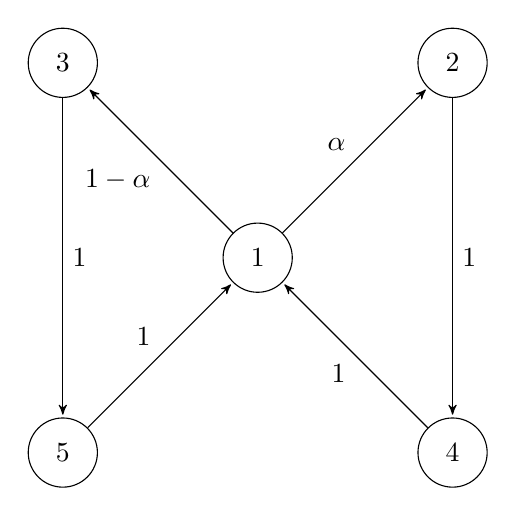
\begin{tikzpicture}[->,>=stealth',shorten >=1pt,auto,node distance=3.5cm]
  \node[state]         (1) {$1$};
  \node[state]         (2) [above right of=1] {$2$};
  \node[state]         (3) [above left of =1] {$3$};
  \node[state]         (4) [below right of=1] {$4$};
  \node[state]         (5) [below left of=1] {$5$};
 
  \path (1)  edge              node {$\alpha$} (2)
             edge              node {$1-\alpha$} (3)
        (2)  edge              node {$1$} (4)
        (3)  edge              node {$1$} (5)
	   (4)  edge              node {$1$} (1)
	   (5)  edge              node {$1$} (1);
\end{tikzpicture}

Inspecting it, we see that $\forall i,j \in S$, $i \leftrightarrow j$ since there is a path between every pair of vertices, so the chain consists of a single closed communicating class.
\item
The chain consists of a single, irreducible, finite closed communicating class, so all states must be positive recurrent.
\item
We can see that there are exactly two cycles for state 1, namely $(1,2,4,1)$ and $(1,3,5,1)$. Both of these cycles are of order 3, so
\begin{align*}
d_1 &= hcf\{3,6,9,12,\dots\}\\
&= 3
\end{align*}
Where $i\leftrightarrow j$, we have that $d_i=d_j$, so $\forall i,j \in S, d_i=d_j=d_1=3$, so
$$
\forall i \in S, d_i = 3
$$
\item
Suppose $\underline{\pi} P = \underline{\pi}$
\begin{align}
\implies \pi_1 &= \pi_4 + \pi_5\\
\pi_2 &= \alpha \pi_1\\
\pi_3 &= (1-\alpha) \pi_1\\
\pi_4 &= \pi_2 \\
\pi_5 &= \pi_3
\end{align}
Any choices of $\pi_2$ and $\pi_3$ would satisfy (4) and (5), so any choice of  $\pi_4$ and $\pi_5$ would satisfy (1). We can then reqrite everything as:
\begin{align*}
\pi_1 &= \pi_1\\
\pi_2 &= \alpha \pi_1\\
\pi_3 &= (1-\alpha) \pi_1\\
\pi_4 &= \alpha\pi_1 \\
\pi_5 &= (1-\alpha)\pi_1 
\end{align*}
We also require that $\sum\limits^5_{i=1}\pi_i=1$, so $3\pi_1 = 1$, and $\pi_1 = \frac{1}{3}$.
$$
\underline{\pi} = \left(\frac{1}{3},\frac{\alpha}{3},\frac{1-\alpha}{3},\frac{\alpha}{3},\frac{1-\alpha}{3}\right) \mbox{ is a stationary distribution.}
$$
\item
No limiting distribution exists, since the chain is periodic and limiting distributions are only defined for aperiodic chains.
\end{enumerate}
\item 
Let $||\underline{x}||_1$ denote $\sum\limits_{i\in\mathcal{X}}x_i$. Suppose $\underline{\mu}$ satisfies $\underline{\mu} Q=\underline{\mu} \wedge ||\underline{\mu}||_1 = 1$
\begin{align*}
\iff \mu_i &= \sum^n_{j=1}q_{ij}\mu_j\\
&= \sum^n_{j=1}\delta p_{ij}\mu_j + (1-\delta)\mu_i \quad \mbox{ since $p_{ii}=0$}\\
\iff \delta \mu_i &= \sum^n_{j=1}\delta p_{ij} \mu_j\\
\iff \mu_i &= \sum^n_{j=1}p_{ij}\mu_j
\end{align*}
So $\underline{\mu}$ satisfies $\underline{\mu}P = \underline{\mu} \wedge ||\underline{\mu}||_1 = 1$, and is therefore a stationary distribution for $P$. All of these steps will also work backwards, so stationary distributions for $P$ are also stationary distributions for $Q$.
\begin{enumerate}
\item
As before, each state intercommunicates, but now state 1 has cycle $(1,1)$ of order 1, so $d_1|1$ and $d_1 | 3$, hence $d_1 =1$, since 1 and 3 are coprime. Similar logic to before will give us that $\forall i \in S, d_i = 1$, so the chane is aperiodic.
\item
Since the chain is aperiodic, a limiting distribution exists and is equal to the stationary distribution, namely:
$$
\underline{\pi} = \left(\frac{1}{3},\frac{\alpha}{3},\frac{1-\alpha}{3},\frac{\alpha}{3},\frac{1-\alpha}{3}\right) \mbox{ is the limiting distribution.}
$$
\end{enumerate}

\end{enumerate}
\end{enumerate}


\end{document}